\documentclass[a4paper]{article}

\usepackage{pdp}

%------------------------------------------------------------------------------
%	REPORT INFORMATION
%------------------------------------------------------------------------------

\title{Quoridor -- Java}
\subtitle{Rapport préliminaire}
\author{Abdeldjabar Ismail Abdraman, Cengiz Vasseur, Joris Douillet, Khadidja Ahmat Hassan, Matthieu Pourageaud}

%------------------------------------------------------------------------------

\begin{document}

%------------------------------------------------------------------------------
%	TITLE PAGE
%------------------------------------------------------------------------------

\maketitle
\thispagestyle{empty}

%------------------------------------------------------------------------------
%	MAIN MATTER
%------------------------------------------------------------------------------


\section{Présentation du sujet et de l'existant}

\subsection{Historique et règles du jeu}

Le Quoridor est un jeu de stratégie abstrait, déterministe et à information parfaite,
conçu par Mirko Marchesi. Il se joue sur un plateau carré de $9 \times 9$ cases, bien
que le projet autorise des variantes allant de $3 \times 3$ à $15 \times 15$ tant que
la taille reste impaire. Le jeu peut opposer deux ou quatre joueurs.

Chaque joueur dispose d'un pion et d'un nombre limité de murs, avec 20 murs au total
répartis selon le nombre de joueurs. L'objectif est d'être le premier à atteindre
n'importe quelle case de la ligne opposée à sa ligne de départ.

À chaque tour, un joueur peut soit déplacer son pion d'une case (horizontalement ou
verticalement), soit poser un mur afin de bloquer la progression des adversaires.
La seule contrainte majeure est l'interdiction de bloquer totalement l'accès d'un
joueur à sa ligne d'arrivée : un chemin libre doit toujours subsister.

La notation utilise les lettres de \texttt{a} à \texttt{i} pour les colonnes (de gauche
à droite) et les chiffres de 1 à 9 pour les lignes (du haut vers le bas).
Par exemple :
\begin{itemize}
    \item \texttt{e2-e3} : déplacement du pion de e2 vers e3
    \item \texttt{e2v} : mur vertical entre les colonnes e et f aux lignes 2 et 3
    \item \texttt{e2h} : mur horizontal entre les lignes 2 et 3 aux colonnes e et f
\end{itemize}

Le symbole \texttt{\_} représente une case vide, \texttt{X} un mur et \texttt{.} les
espaces verticaux entre deux cases.

Il est également possible de sauter par-dessus un pion adverse si une case libre
existe derrière celui-ci, sous réserve de l'absence de mur bloquant le mouvement. Les murs rouges dans l'image suivante représentent donc les murs invalides.

\begin{figure}[H]
    \centering
    \begin{minipage}{0.45\textwidth}
        \centering
        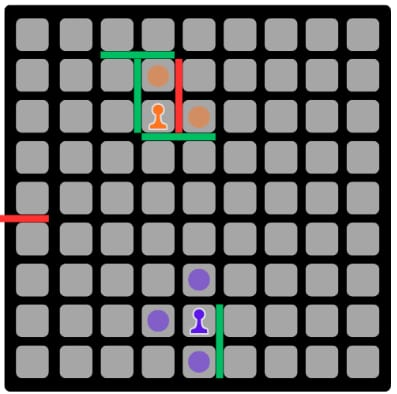
\includegraphics[width=\linewidth]{interdit.jpeg}
        \caption{Murs interdits}
        \label{fig:murs_interdits}
    \end{minipage}
    \hfill % Crée un espace élastique entre les deux blocs
    \begin{minipage}{0.45\textwidth}
        \centering
        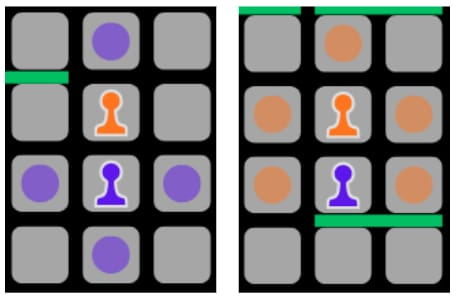
\includegraphics[width=\linewidth]{Saut_joueur.jpeg}
        \caption{Saut par dessus un joueur}
        \label{fig:saut_joueur}
    \end{minipage}
\end{figure}

\subsection{Analyse de la complexité du jeu}


Le \emph{Quoridor} est classé parmi les jeux à haute complexité combinatoire, se
situant entre les échecs et le jeu de Go en raison de la nature hybride de ses coups.

Le plateau comporte 81 cases. Avec deux pions, on obtient :
\[
81 \times 80 = 6480
\]
positions distinctes.

Il existe 64 points d'intersection pour les murs, chacun pouvant être orienté 
verticalement ou horizontalement, soit 128 possibilités. En prenant en compte 
20 murs, et en utilisant la formule de Mertens :
\begin{equation}
S_f = \sum_{n=0}^{20} \left( \prod_{i=0}^{n-1} (128 - 4i) \right)
\end{equation}
on peut estimer la complexité de l'espace d'états à environ $10^{42}$ \cite{mertens2006}.

Le facteur de branchement moyen est estimé à $\sim 60$ \cite{glendenning2005}, contre 35
pour les échecs. Une partie dure en moyenne 100 demi-coups, ce qui donne une
complexité totale de l'arbre de jeu de :
\[
60^{100} \approx 10^{177}
\]


\subsection{État de l'art et apports du projet}

Le Quoridor possède de nombreuses adaptations numériques, notamment sur des
plateformes web comme \emph{Board Game Arena}. Des travaux académiques majeurs,
tels que ceux de Glendenning (2005) et Mertens (2006), ont formalisé les premières
notations algébriques et heuristiques.

L'objectif de ce projet est de proposer une plateforme unifiée cherchant à combler l'écart entre les travaux académiques théoriques et les applications ludiques actuelles, souvent limitées à une interface unique ou à une intelligence artificielle simpliste. L'implémentation vise à intégrer un moteur de décision multi-paradigme combinant le Minimax avec élagage alpha-bêta, la recherche arborescente Monte Carlo (MCTS) et l'apprentissage automatique au sein d'une architecture modulaire robuste. En complément des standards ergonomiques actuels, le projet met l'accent sur une double interface (graphique et console interactive) ainsi que sur une infrastructure réseau asynchrone incluant la découverte dynamique de serveurs par broadcast UDP. Cette approche permet de garantir une fiabilité logicielle élevée, validée par une couverture de tests automatisés systématiques.

\section{Algorithmes et structures de données}

\subsection{Modélisation du plateau par graphe}

Le plateau est modélisé par un graphe non orienté $G = (V, E)$ où chaque sommet
représente une case du plateau et chaque arête un déplacement possible.

Une liste d'adjacence est utilisée car le graphe est peu dense (au plus 4 voisins par
sommet), ce qui permet une complexité mémoire en $O(V + E)$ et un accès en temps
constant aux voisins.

Les sommets sont indexés de 0 à 80 selon la formule :
\[
index = ligne \times 9 + colonne
\]

Les murs ne sont pas représentés comme des sommets, mais comme des contraintes
invalidant certaines transitions.

\subsection{Algorithmes de recherche de chemin}

Le graphe étant non pondéré, un parcours en largeur (BFS) est utilisé pour calculer
la distance minimale entre un pion et sa ligne d'arrivée. Cette information est
utilisée pour la détection de victoire et les fonctions d'évaluation du Minimax.

Une vérification de connexité est également effectuée lors du placement des murs
afin de garantir qu'un chemin valide subsiste toujours.

\subsection{Stratégies d'intelligence artificielle}

Le Quoridor étant un jeu à information parfaite et déterministe, l'implémentation de joueurs artificiels repose sur des méthodes de recherche arborescente visant à explorer l'explosion combinatoire générée par le placement des murs.\cite{lloyd2022}

\subsubsection{Minimax avec élagage alpha-bêta}

L’algorithme Minimax est une méthode de prise de décision issue de la théorie des jeux pour les jeux à deux joueurs à information complète (comme le Quoridor ou les Échecs). Son objectif est de déterminer le coup optimal en anticipant les réactions rationnelles de l'adversaire. Le Minimax repose sur une exploration récursive de l’arbre des possibles, où chaque niveau de l'arbre représente le tour d'un joueur, le joueur “MAX” cherche à maximiser son score tandis que le joueur “MIN” cherche à minimiser son score. L’algorithme descend dans l’arbre jusqu’à une profondeur déterminée. Une fois à cette profondeur, des fonctions d’évaluation sont utilisées pour évaluer les positions aux feuilles de l'arbre, trois fonctions d'évaluation distinctes sont implémentées, basées notamment sur les distances minimales calculées via le module graph et la gestion des réserves de murs.\\
Pour rendre l’algorithme meilleur, on utilise la technique d’optimisation d’élagage Alpha-Beta qui permet de ne pas explorer les branches dont on sait qu’elles n’influenceront pas le choix final. L’Alpha est le score minimum obtenable et Beta est le score maximum obtenable. Si, lors de l'exploration, l'algorithme découvre une branche où le score est inférieur à Alpha ou supérieur à Beta, il "coupe" (élague) cette branche. Cela permet de doubler, voire tripler la profondeur de recherche pour un même temps de calcul.


\begin{figure}[H]
    \centering
    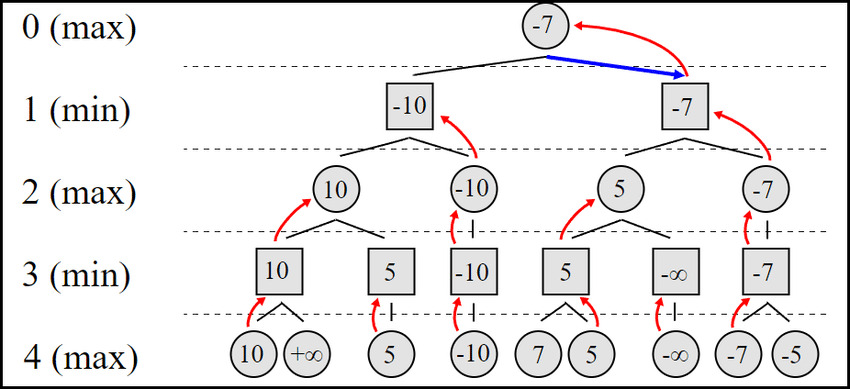
\includegraphics[width=0.8\linewidth]{MiniMax.jpg}
    \caption{Exemple de MiniMax}
    \label{fig:minimax}
\end{figure}

\subsubsection{Monte Carlo Tree Search}

Un algorithme de \emph{Monte Carlo Tree Search} (MCTS) est également implémenté.
L'algorithme MCTS repose sur quatre phases : sélection, expansion, simulation et mise
à jour. Contrairement à l’algorithme Minimax, qui explore l’arbre de jeu de manière
exhaustive jusqu’à une profondeur fixe, le MCTS repose sur une approche
probabiliste et statistique. Ce choix est particulièrement pertinent pour le jeu
\emph{Quoridor}, dont le facteur de branchement élevé rend une exploration complète
de l’arbre de jeu extrêmement coûteuse en temps de calcul.

Selon les travaux de Browne \emph{et al.}~\cite{browne2012}, l’algorithme MCTS progresse
de manière itérative à travers quatre phases fondamentales :

\begin{itemize}
    \item \textbf{Sélection} : l’intelligence artificielle parcourt l’arbre des
    décisions déjà construit en choisissant le chemin jugé le plus prometteur.
    Ce choix est guidé par la fonction UCT (\emph{Upper Confidence bounds applied
    to Trees}), qui permet de favoriser les branches les plus performantes tout
    en conservant une part d’exploration pour les alternatives.

    \item \textbf{Expansion} : lorsque l’algorithme atteint un état du jeu encore
    partiellement exploré, correspondant à une feuille de l’arbre, un nouveau
    coup légal est ajouté, créant ainsi une nouvelle branche à analyser.

    \item \textbf{Simulation} : à partir de cette nouvelle branche, l’IA termine
    la partie de manière entièrement aléatoire afin d’obtenir un résultat
    (victoire ou défaite).

    \item \textbf{Mise à jour} : une fois la simulation achevée, le résultat est
    propagé vers la racine de l’arbre en mettant à jour les statistiques des
    nœuds parcourus, permettant d’évaluer la qualité du coup testé.
\end{itemize}

Lorsque le temps de calcul alloué est écoulé (ou qu’un nombre maximal
d’itérations est atteint), l’algorithme entre dans sa phase de décision finale.
Le coup sélectionné correspond alors au nœud ayant été le plus fréquemment visité
au cours des simulations. En effet, la formule UCT oriente naturellement
l’exploration vers les branches les plus performantes, faisant du nombre de
visites un indicateur fiable de la supériorité statistique d’un coup.

\begin{figure}[H]
    \centering
    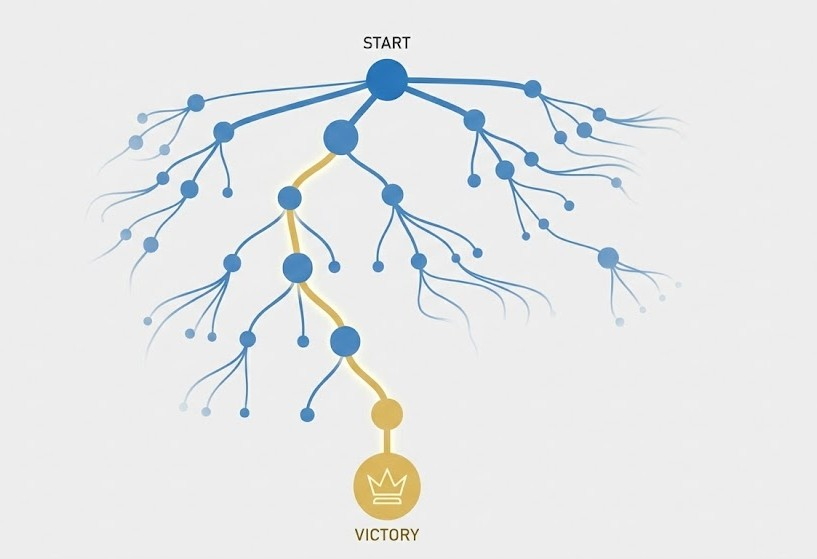
\includegraphics[width=0.5\linewidth]{MCTS_image.jpg}
    \caption{MCTS Représentation}
    \label{fig:mcts}
\end{figure}


\subsubsection{Apprentissage automatique}

Un modèle de Machine Learning est intégré pour guider la sélection des coups dans le MCTS. Les variables utilisées incluent la distance à l'arrivée et le nombre de murs restants pour chaque joueur.

Pour optimiser les performances du \emph{Monte Carlo Tree Search} (MCTS), une
fonction de sélection basée sur l'apprentissage automatique est intégrée.
Contrairement à l'approche classique qui traite tous les coups inconnus de manière
uniforme lors de la phase de sélection, l'intelligence artificielle utilise ici un
modèle prédictif (de type régression logistique ou arbre de décision) afin d'estimer
la probabilité de victoire associée à chaque coup, avant même le lancement des
simulations.

L'utilisation du \emph{Machine Learning} permet ainsi de remplacer le caractère
purement aléatoire du MCTS en priorisant les coups présentant un potentiel
stratégique plus élevé. Pour estimer la probabilité de victoire d'un coup, un réseau
de neurones est employé. Les entrées de ce réseau correspondent aux principales
variables stratégiques du jeu, à savoir :
\begin{itemize}
    \item la distance restante à la ligne d'arrivée pour chacun des deux joueurs ;
    \item le nombre de murs encore disponibles pour chaque joueur.
\end{itemize}

Durant la phase d'apprentissage, le réseau ajuste ses poids internes afin de
comprendre l'influence relative de ces variables sur l'issue d'une partie. Par
exemple, il peut apprendre qu'une faible réserve de murs peut être compensée par
une distance très courte à la ligne d'arrivée.

En remplaçant le pur hasard par cette expertise statistique, l'intelligence
artificielle gagne significativement en efficacité : elle priorise les branches
stratégiquement solides et converge beaucoup plus rapidement vers le coup optimal,
même en présence d'un facteur de branchement élevé.

% =====================================================
\section{Choix de l’architecture}
\subsection{Justification du choix d’architecture
}
Le projet Quoridor nécessite l’implémentation d’un moteur de jeu respectant
des règles strictes, tout en supportant plusieurs modes d’interaction (interface
en ligne de commande, interface graphique, intelligence artificielle et jeu en
réseau). Ces contraintes impliquent une forte complexité métier, une exigence
de fiabilité des règles et une capacité d’évolution du logiciel. Afin de répondre à ces objectifs, nous avons retenu une architecture modulaire orientée
domaine, inspirée de la Clean Architecture (Ports \& Adapters) \cite{martin2017clean}.\\

Notre système est organisé autour d’un cœur métier central (core) qui regroupe
l’ensemble de la logique du jeu : règles, état de la partie, moteur d’exécution
et entités principales. Ce module est totalement indépendant des autres modules garantissant que la logique métier reste cohérente,
testable et inchangée quelles que soient les modalités d’interaction avec le
jeu.\\

Les modules complémentaires (cli, gui, network, persistence, config, i18n) fonctionnent comme des adaptateurs qui interagissent avec le cœur via des interfaces bien définies. Cette organisation permet de changer, ajouter ou supprimer des interfaces sans impacter la logique du jeu. Par exemple, l’IA (modules ai/minimax ou ai/mcts) peut simuler des parties en utilisant directement le GameState et le Board sans dépendre de l’interface graphique ou de la CLI.

Le patron MVC (Model–View–Controller) est utilisé uniquement au niveau des
interfaces. Le module core correspond au modèle, tandis que les modules cli
et gui implémentent les vues et contrôleurs. Cette utilisation locale de MVC
permet de séparer clairement la présentation de la logique métier sans
imposer ce modèle à l’ensemble de l’architecture.\\

Ce choix architectural apporte plusieurs bénéfices : une maintenabilité
accrue, une testabilité élevée du moteur de jeu, une extensibilité facilitée
(ajout de nouvelles IA ou interfaces) et une robustesse globale, puisque
toutes les actions passent nécessairement par la validation des règles du
cœur métier. Cela constitue un
compromis efficace entre rigueur logicielle, évolutivité, lisibilité du code, et est adaptée à un projet de jeu à règles complexes comme Quoridor.

\subsection{Schémas de l'architecture}

\begin{figure}[H]
    \centering
    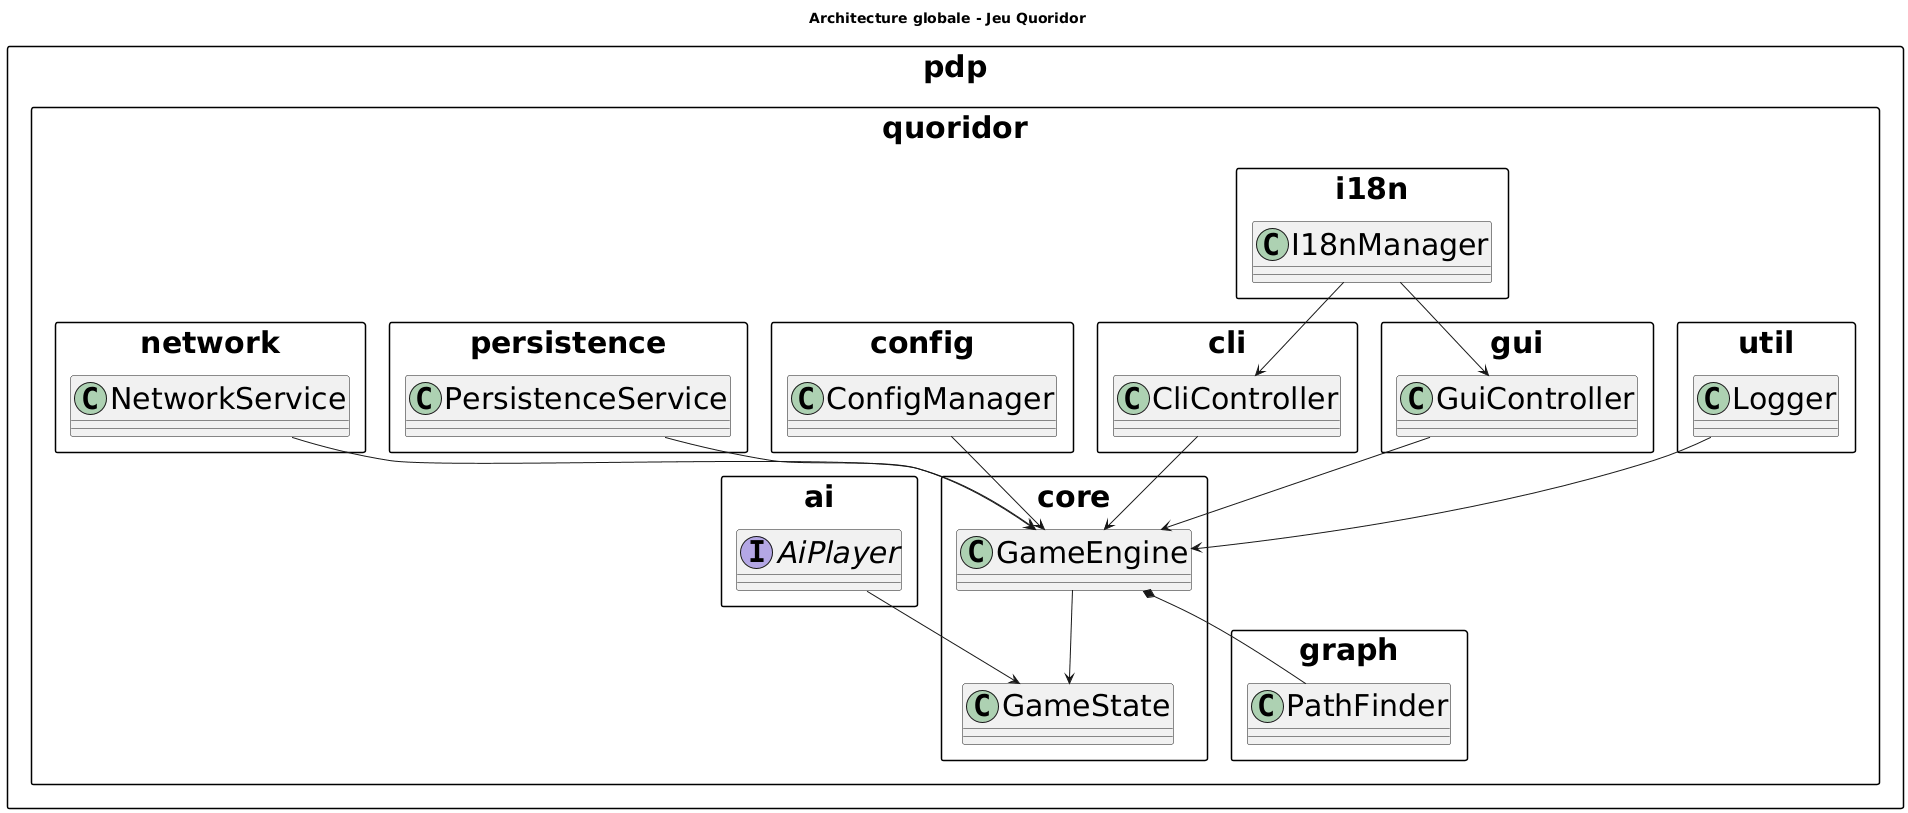
\includegraphics[width=0.75\textwidth]{Architecture global pdp pre.png}
    \caption{Schéma global de l’architecture}
    \vspace{0.5cm} % Un peu d'espace entre les deux
    
    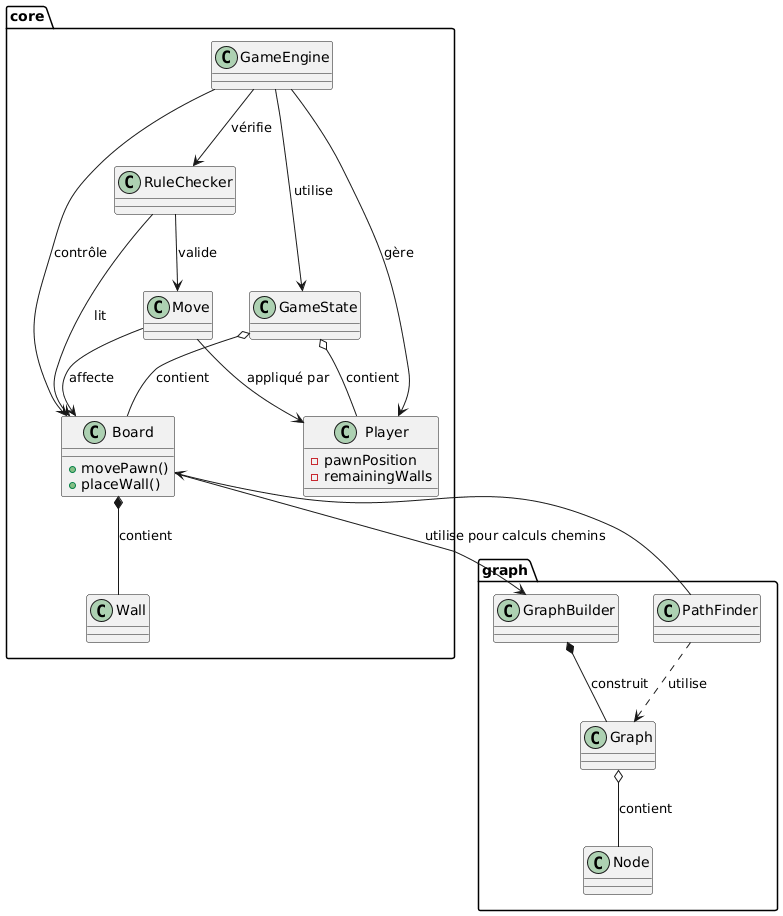
\includegraphics[width=0.82\textwidth]{uml core + graph en detaile.png}
    \caption{Schéma d'UML core + graph en détaillé}
    \label{fig:architectures_groupees}
\end{figure}


\section{Spécification étendue : MiniMax}

\subsection{Prérequis}
L'implémentation de cet algorithme s'appuie sur plusieurs besoins :
\begin{itemize}
    \item \textbf{F33 (Heuristiques) :} Nécessité de fonctions d'évaluation pour quantifier l'avantage d'un plateau donné.
    \item \textbf{F8 (Mode IA) :} Cadre global permettant l'exécution et le test de l'algorithme.
    \item \textbf{F10 (Gestion des règles) :} Fournit la liste des coups légaux via le moteur de jeu, condition sine qua non pour l'exploration de l'arbre.
    \item \textbf{F31 (Temps de réflexion borné) :} Mécanisme de contrôle pour interrompre l'exploration si la profondeur de recherche excède le temps imparti.
\end{itemize}

\subsection{Fonctions requises et signatures}
Le bon fonctionnement du MiniMax repose sur la collaboration entre le moteur de jeu (\texttt{core}) et le module d'intelligence artificielle (\texttt{ai}). Il est obligatoire d’avoir au moins une fonction heuristique (qui sera implémentée par F37.) ainsi qu’une fonction getPossibleMoves () retournant les coups possibles à jouer. C’est grâce à ces fonctions que nous allons pouvoir implémenter 2 autres fonctions qui vont permettre la résolution de ce besoin, qui sont MinMax() et MaxMin().\\

Les signatures principales retenues sont les suivantes :
\begin{itemize}
    \item \texttt{public ArrayList<Move> getPossibleMoves(Player p)} \\ \textit{(Méthode de la classe Board, module core)}
    \item \texttt{public int evaluate(Board b)} \\ \textit{(Fonction heuristique, module ai)}
    \item \texttt{public int minMax(Board b, int depth, int alpha, int beta)}
    \item \texttt{public int maxMin(Board b, int depth, int alpha, int beta)}
\end{itemize}

\subsection{Architecture et Dépendances}
Conformément à notre architecture modulaire, le besoin prend forme essentiellement dans le package \texttt{ai}.
\begin{itemize}
    \item \textbf{Localisation :} Les algorithmes de décision et les fonctions d'évaluation résident dans \texttt{ai}.
    \item \textbf{Dépendances :} Ce module dépend exclusivement du package \texttt{core}. Il utilise les objets \texttt{Board}, \texttt{Player} et \texttt{Move} pour simuler les états futurs du jeu sans impacter l'état réel de la partie en cours.
\end{itemize}

\subsection{Stratégie de tests}
Pour valider l'efficacité du MiniMax, deux protocoles de test sont mis en place :
\begin{enumerate}
    \item \textbf{Test de Sanité :} Confrontation contre un joueur jouant aléatoirement. L'algorithme doit systématiquement l'emporter, démontrant que sa prise de décision est supérieure au hasard.
    \item \textbf{Test de Performance (Profondeur) :} Confrontation de deux instances du MiniMax avec des profondeurs de recherche différentes (ex: profondeur 2 vs profondeur 4). Le résultat attendu est une victoire de l'instance disposant de la plus grande profondeur d'anticipation.
\end{enumerate}

%------------------------------------------------------------------------------
%	BIBLIOGRAPHY
%------------------------------------------------------------------------------

\nocite{*}
\bibliographystyle{plain}
\bibliography{bibliography}

%------------------------------------------------------------------------------
% BACK MATTER
%------------------------------------------------------------------------------
\appendix


\end{document}
